\documentclass[11pt, letterpaper]{article}
\usepackage[utf8]{inputenc}
\usepackage[letterpaper, margin=0.5in]{geometry}
\usepackage{amsmath}
\usepackage{amssymb}
\usepackage{amsthm}
\usepackage{graphicx}
\usepackage[font=scriptsize]{caption}
\usepackage{subcaption}
\graphicspath{ {.} }
\captionsetup{justification=raggedright, singlelinecheck=false}


\title{STA 602 HW2}
\author{Ryan Tang}
\date{September 30th 2022}

\begin{document}
\maketitle

\section{Exercise PH 3.9}
\paragraph{(a)}
We can express the Galenshore distribution in its exponential family form, and assuming $a$ is a constant makes things simpler.
First, Galenshore's kernel has the following form.
\begin{align*}
    Galenshore \thicksim p(y|a, \theta)
        &= \frac{2}{\Gamma(a)} \theta^{2a} y^{2a-1} e^{-\theta^2 y^2} \\
        &\propto y^{2a-1} e^{-\theta^2 y^2}
\end{align*}
Second, we write it in the exponential family format under the condition that all parameters are positive.
\begin{align*}
    p(y|a, \theta)
        &= \frac{2}{\Gamma(a)}\theta^{2a} \exp [(2a-1) \log y - \theta^2 y^2] \\
    h(y) &= y^{2a-1} \quad c(\eta) = \frac{-2}{\Gamma(a)}\eta^a \quad
    \eta = -\theta^2 \quad t(y) = y^2 \\
    p(y|\eta) &= h(y) c(\eta) \exp[\eta t(y)]
\end{align*}
Therefore, $\eta$ has a conjugate prior in the exponential family with the following form. And, we can retrieve the prior in terms of $\theta$ using change of variable. 
\begin{align*}
    p(\eta|n_0, t_0) &\propto c(\eta)^{n0} \exp[\eta n_0 t_0] \\
    p(\theta|n_0, t_0)
        &\propto (\frac{2}{\Gamma(a)}\theta^{2a})^{n_0} \exp[-\theta^2 n_0 t_0] \cdot |-2\theta| \\
        &\propto \theta^{2a n_0 + 1} e^{-\theta^2 n_0 t_0}
\end{align*}
Here if we view $\theta$ just like $y$, we get a Galenshore distribution after some algebra solving the values for the two parameters. Hence, the conjugate prior is a Galenshore distribution for the Galenshore sampling model. See Figure 1 for density plot with various parameters.
\begin{align*}
    p(\theta) &\thicksim Galenshore(\alpha=an_0 +1, \beta=\sqrt{n_0 t_0}) \\
        &= \frac{2}{\Gamma(\alpha)} \beta^{2\alpha}\theta^{2\alpha-1}e^{-\theta^2 \beta^2}
\end{align*}

\begin{figure*}[!h]
  \centering
  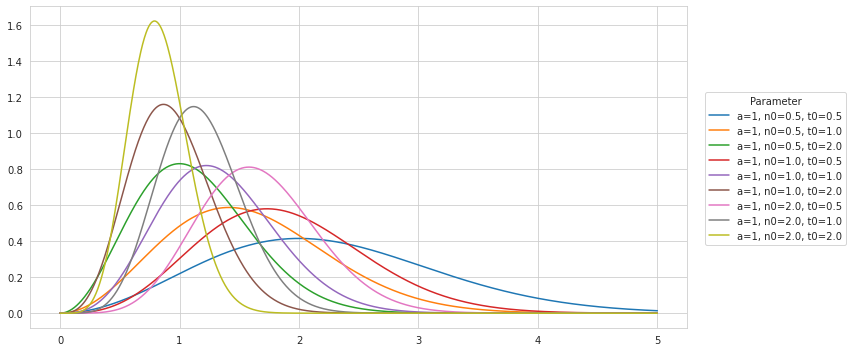
\includegraphics[width=0.9\textwidth]{1.a.png}
  \captionsetup{justification=centering}
  \caption{Galenshore Prior Parameterized by $n_0$ and $t_0$}
\end{figure*}

\paragraph{(b)}
Given the iid sampling model, here is the posterior, which follows the typical exponential family updates.
\begin{align*}
    p(Y|\theta)
        &= \prod_i p(y_i|\theta) \\
        &= (\frac{2}{\Gamma{a}} \theta^{2a})^n \exp[(2a-1) \sum_i \log y_i - \theta^2 \sum_i y_i^2] \\
    p(\theta|Y) &\propto p(Y|\theta) p(\theta) \\
        &=
            (\frac{2}{\Gamma{a}})^n \theta^{2an} \exp[(2a-1) \sum_i \log y_i] e^{- \theta^2 \sum_i y_i^2}
            \frac{2}{\Gamma(an_0 + 1)} (n_0 t_0)^{2a n_0 + 2} \theta^{2an_0+1} e^{-\theta^2 n_0 t_0} \\
        &\propto \theta^{2a(n_0+n)+1} e^{-\theta^2(n_0 t_0 + \sum_i y_i^2)} \\
        &\thicksim Galenshore(\alpha = a (n_0+n) + 1, \beta = \sqrt{n_0 t_0 + \sum_i y_i^2})
\end{align*}

\paragraph{(c)}
As we would expect that the Galenshore distribution, which belongs to the exponential family, has sufficient statistics given by $t(y) = y^2$.
\begin{proof}
\begin{align*}
    \frac{p(\theta_1|Y)}{p(\theta_2|Y)}
        &= \frac{{\theta_1}^{2a(n_0+n)+1} \exp[-(n_0t_0+\sum_i y_i^2)\theta_1^2]}{{\theta_2}^{2a(n_0+n)+1} exp[-(n_0t_0+\sum_i y_i^2)\theta_2^2]} \\
        &= ({\frac{\theta_1}{\theta_2}})^{2a(n_0+n)+1} \exp[-(n_0t_0+\sum_i y_i^2)(\theta_1^2 - \theta_2^2)]
\end{align*}
\end{proof}

\paragraph{(d)}
\begin{align*}
    E[\theta|Y] = \frac{\Gamma(a(n_0+n)+3/2)}{\Gamma(a(n_0+n)+1) \sqrt{n_0t_0 + \sum_i y_i^2}}
\end{align*}

\paragraph{(e)}
The general form of the posterior predictive density is given below.
\begin{proof}
\begin{align*}
    p(\tilde{y}|Y) &= \int p(\tilde{y}|\theta, Y) p(\theta|Y) d\theta \\
        &= \int p(\tilde{y}|\eta, Y) p(\eta|Y) d\eta \\
        &= \int h(\tilde{y})c(\eta)\exp[\eta t(\tilde{y})] \cdot \kappa(\alpha, \beta)c(\eta)^{n_0+n} \exp[\eta(n_0t_0+n\bar{t}(Y)] d\eta \\
        &= h(\tilde{y}) \kappa(\alpha, \beta) \int c(\eta)^{n_0+n+1} \exp[\eta(n_0t_0+n\bar{t}(Y)+t(\tilde{y})] d\eta \\
        &= h(\tilde{y}) 
            \frac{\kappa(\alpha=a(n_0+n)+1, \beta=\sqrt{n_0t_0 + \sum_i y_i^2})}
                 {\kappa(\alpha=a(n_0+n+1)+1, \beta=\sqrt{n_0t_0 + \sum_i y_i^2 + \tilde{y}^2})} \\ \\
    \kappa &= \frac{2}{\Gamma(\alpha)} \beta^{2\alpha} \quad h(y) = y^{2a-1}
\end{align*}
\end{proof}
\newpage

\section{Exercise 2}
\paragraph{(a)}
Given the $\theta|X$ posterior, we can write the Bayes estimator and the resulting MSE with the following form.
\begin{align*}
    \theta &\thicksim Gamma(a=10, b=1) \\
    \theta|X &\thicksim Gamma(a=210, b=11) \\
    X &\thicksim Poisson(\theta) \\
    \delta_{bayes}(X) &= \frac{X+10}{n+1} && X=200 \quad n=10 \\ \\ 
    \text{MSE}(\delta_{bayes}(X), \theta) &= \mathbb{E}[(\delta(X) - \theta)^2|\theta] \\
        &= \text{Var}(\frac{X+10}{n+1}) + (\mathbb{E}[\frac{X+10}{n+1}] - \theta)^2 \\
        &= \frac{\sum_i \mathbb{E}[X_i|\theta]}{(n+1)^2} + (\frac{\sum_i \mathbb{E}[X_i] + 10}{n+1} - \theta)^2\\
        &= \frac{n\theta}{(n+1)^2} + (\frac{n\theta + 10}{n+1} - \theta)^2 \\
        &= \text{Variance} + \text{Bias}^2
\end{align*}

\paragraph{(b)}
When the true $\theta$ lies between the $[6.25, 15.5]$ range, the Bayes estimator tends to have an overall lower MSE than the MLE estimator.mainly mostly because the MLE estimator tends to have higher variances. Hence, some bias in Bayes estimator can actually improve the general prediction. It is also because we have a relatively small sample size, $n = 10$.

\begin{figure*}[!h]
  \centering
  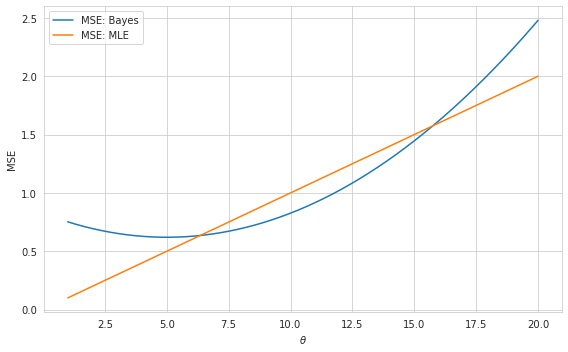
\includegraphics[width=0.65\textwidth]{2.a.png}
  \captionsetup{justification=centering}
  \caption{MSE Comparison}
\end{figure*}


\section{Exercise 3}
\paragraph{(a)}
The MSE and its corresponding variances and biases decomposition for estimator $\delta_5$ are as follows.
\begin{align*}
    \delta_5(X) &= \frac{X+\sqrt{n}/2}{n + \sqrt{n}} && X \thicksim Binomial(n, \theta) \\ 
    \text{MSE}(\delta_5(X), \theta) &= \mathbb{E}[(\delta_5(X) - \theta)^2 | \theta] \\
        &= \text{Var}[\frac{X+\sqrt(n)/2}{n + \sqrt{n}}] + (\mathbf{E}[\frac{X+\sqrt{n}/2}{n + \sqrt{n}}] - \theta)^2 \\
        &= \frac{\text{Var}(X)}{(n+\sqrt{n}^2} + (\frac{\mathbf{E}[X] + \sqrt{n}/2}{n + \sqrt{n}} - \theta)^2 \\
        &= \frac{n\theta(1-\theta)}{(n+\sqrt{n})^2} + (\frac{n\theta + \sqrt{n}/2}{n+\sqrt{n}} - \theta)^2
\end{align*}

\paragraph{(b)}
I have plotted all MSE concerning the true $\theta$ for the comparison below (Figure 3 and Figure 4). We can see that the $\delta_5$ estimator performs similarly to the uniform prior estimator when the data size is small. However, even when we increased $n$ to 100, the MSE generated from the $\delta_5$ is still quite flat. In other words, it is relatively invariant to the sample size.

\begin{figure*}[!h]
  \centering
  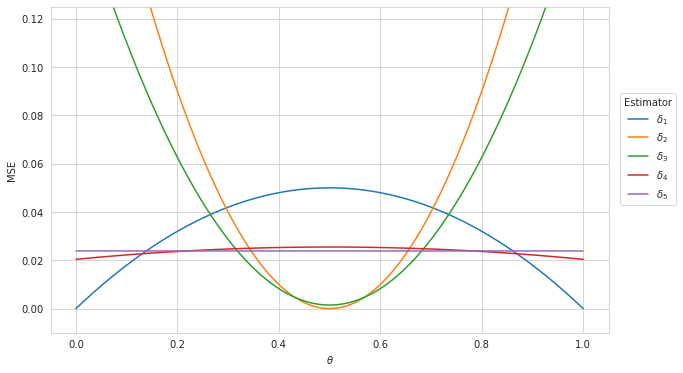
\includegraphics[width=0.7\textwidth]{3.b.png}
  \captionsetup{justification=centering}
  \caption{Political Poll MSE Comparison, $n = 5$}
\end{figure*}

\begin{figure*}[!h]
  \centering
  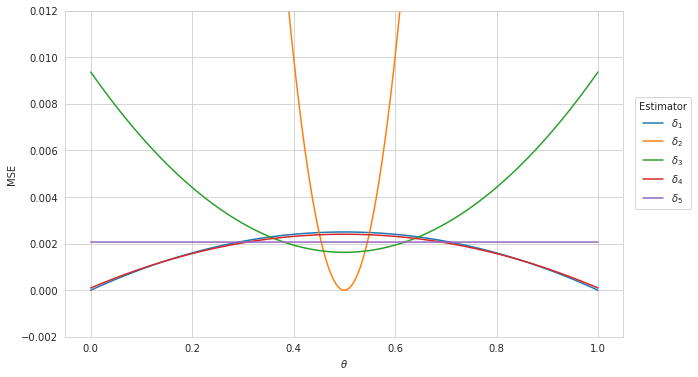
\includegraphics[width=0.7\textwidth]{3.b.2.png}
  \captionsetup{justification=centering}
  \caption{Political Poll MSE Comparison, $n = 100$}
\end{figure*}

\paragraph{(c)}
We can write $\delta_5$ in terms of $\delta_1$ and $\delta_2$. We can see it puts a square root of weight on the prior. With a typical Bayesian prior, the weights are constant so that with sufficient data, it can wash away the prior effect. However, in the case of $\delta_5$, we are putting more weight on the prior the more data we have. Hence it prolongated the prior effect. I think that is why it is called the minimax estimator. It minimizes the maximum risk.
\begin{align*}
    \delta_5 &= \frac{n}{n + \sqrt{n}} \delta_1 + \frac{\sqrt{n}}{n+\sqrt{n}} \delta_2
\end{align*}

\paragraph{(d)}
Now instead of plotting MSE, here we estimated MAE using Monte Carlo. Still the same 5 estimators, below are the MAE comparisons (Figures 5 and 6). I noticed that the loss function is longer convex; many humps can make optimization stuck in a local maxima. However, the general Bayesian update behaviors stay directionally similar. Lastly, it looks like the $\delta_5$ L2 minimax estimator is still a minimax estimator in the L1 context.
\begin{figure*}[!h]
  \centering
  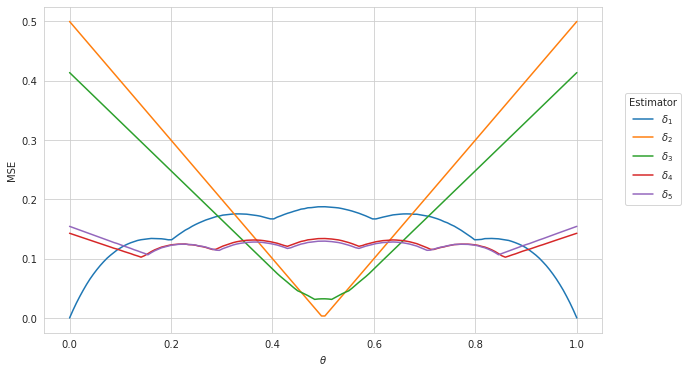
\includegraphics[width=0.7\textwidth]{3.d.1.png}
  \captionsetup{justification=centering}
  \caption{Political Poll MAE Comparison, $n = 5$}
\end{figure*}

\begin{figure*}[!h]
  \centering
  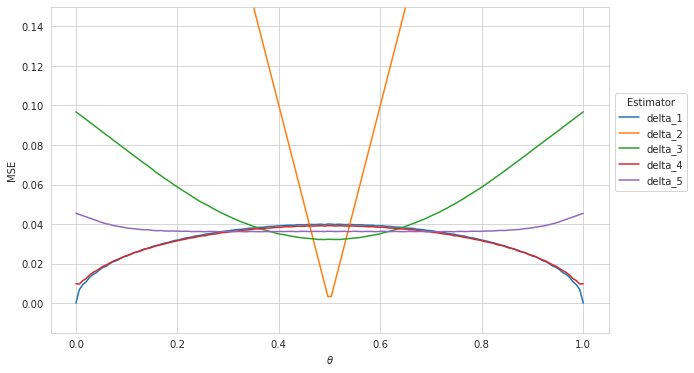
\includegraphics[width=0.7\textwidth]{3.d.2.png}
  \captionsetup{justification=centering}
  \caption{Political Poll MAE Comparison, $n = 100$}
\end{figure*}

\end{document}